\chapter{TEST GENERATION}
\label{chapter:test_generation}

\section{Off-line Test Generation with Graphwalker}
\par
User needs to have Java version 7 or 8 installed on the machine for test generation with Graphwalker. The off-line generation is supported via command line interface, where user needs to pass models and generation criteria as parameters to Graphwalker .jar file. User can generate tests from single as well as from multiple models simultaneously. The example usage is listed below.

\begin{lstlisting}
For single model:
java -jar graphwalker.jar offline -m Login.graphml random(edge_coverage(100))
\end{lstlisting}
\begin{lstlisting}
For multiple models:
java -jar graphwalker.jar offline 
-m src/test/resources/graphml/shared_state/Model_A.graphml random(edge_coverage(100)) 
-m src/test/resources/graphml/shared_state/Model_B.graphml random(edge_coverage(100))
-m src/test/resources/graphml/shared_state/Model_C.graphml random(edge_coverage(100))
-m src/test/resources/graphml/shared_state/Model_D.graphml random(edge_coverage(100))
\end{lstlisting}

\par
Generated tests are given in form of sequence of edges and vertexes and can be observed in the listing below.

\begin{lstlisting}
e_Init
v_ClientNotRunning
e_StartClient
v_LoginPrompted
e_InvalidCredentials
v_LoginPrompted
e_ValidPremiumCredentials
v_Browse
e_Logout
\end{lstlisting}

\par
Graphwalkers allows off-line test generation for from models with multiple selection criteria.  The general pattern for test selection criteria can be observed in figure \ref{Fig:raphwalker_testselection_example}.

\begin{figure} [htbp!]
	\centering
					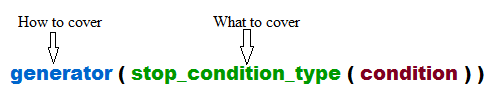
\includegraphics[width=1\textwidth]{figures/Graphwalker_testselection_example.png}
					\caption{\label{Fig:raphwalker_testselection_example} Graphwalker Test Selection pattern}
\end{figure}
\par
As reader can observe, selection criterion consists of generator, stop condition type and condition. Generator stands for the coverage algorithm which takes stop condition type as a parameter. Stop condition type gives Graphwalker information about what exactly to cover using the coverage algorithm. Condition might vary depending on stop condition type.

\subsection{Generator Algorithms}
\par
One of the generator algorithms in Graphwalker is random. This is the algorithm which will be used most extensively for test generation in this thesis. It is also known with name Drunkard's walk or Random walk. This algorithm selects edges not blocked by guards coming out of vertex completely randomly during traversal and continues doing same until stop condition is met. As a parameter it can take multiple stop conditions such as edge or vertex coverage. Examples of its usage can be observed below. 
\begin{lstlisting}
random(vertex_coverage(100))
random(never)
random(reached_vertex(v_SomeVertex))
random(reached_vertex(v_SomeVertex) and edge_coverage(100))
random((reached_vertex(v_SomeVertex) and vertex_coverage(100)) || time_duration(500))
\end{lstlisting}

\par
Weighted\_random coverage does exactly same as random algorithm, but takes into consideration weight annotations on edge labels and decides on next edge based on these weights. Basically, higher the edge weight, more likely it is that Graphwalker will take that edge when its source vertex is reached. It is extremely useful when company has usage profiles of application from customers, so they can test more extensively features which are used more often. Example usage of it would be also same as in case of random, but instead of random keyword we use weighted\_random.

\par
Quick-random tries to cover model with the shortest path. It marks already taken edges 
as visited and tries not to take them any more if there is other option available. Problem is that it does not work with \acrshort{efsm} and might take an edge which is blocked by guard. That is the reason why it cannot be used in our case as most of edges in our models are annotated with guards. Example usage would look exactly same as random but with the keyword quick\_random.

\par
A\_Star algorithm can be used for generating shortest path to an edge or vertex in model. In this case passed stop condition needs to specify which edge or vertex needs to be reached. The example usage can be found below.

\begin{lstlisting}
a_star(reached_edge(e_SomeEdge))
a_star(reached_vertex(v_SomeVertex))
\end{lstlisting}

\subsection{Stop Conditions}
\par
Edge and vertex coverage are the most used stop conditions for any type of random algorithm in Graphwalker. They take as a parameter integer which stands for percentage. So, random(edge\_coverage(95)) would mean that Graphwalker can stop only after it covers 95\% of the edges.

\par
Reached vertex or edge stop condition tells Graphwalker to stop generation when specific edge or vertex which was passed to it as an argument is reached while traversal. For example, a\_star(reached\_vertex(v\_SomeVertex)) would mean that traversal should stop when vertex with name v\_SomeVertex is reached.

\par
Other stop conditions are also provided, such as never stopping the traversal, length of generated sequence, time duration for how long traversal should continue, dependency and requirement coverage, but none of them will be used in scope of this thesis.

\section{Graphwalker GUI}
\par
To simplify test generation even more, instead of command line parameters, we decided to provide \acrshort{gui} for off-line test generation, which you can observe in figure \ref{Fig:Graphwalker_GUi}.

\begin{figure} [htbp!]
	\centering
					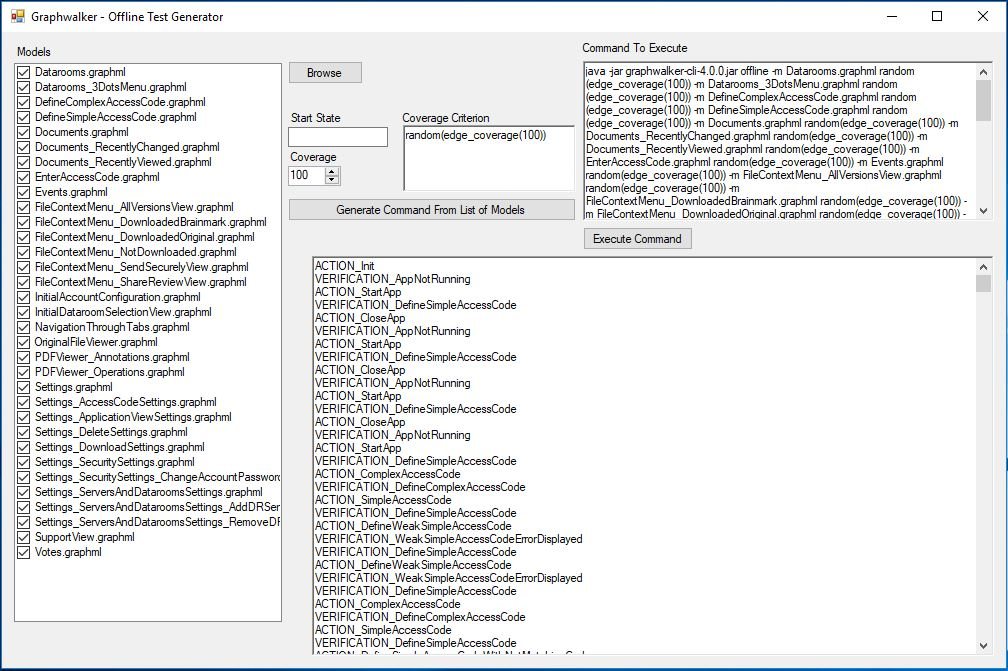
\includegraphics[width=0.95\textwidth]{figures/Graphwalker_GUI_screenshot}
					\caption{\label{Fig:Graphwalker_GUi} Graphwalker Off-line Test Generator}
\end{figure}

\par
Program is based on Windows Forms. User needs to browse the folder where all models reside together with graphwalker .jar file. Then he/she needs to select interesting for him/her models and type coverage criterion. Unfortunately, for now it is only possible to generate command with one coverage criterion for all models, but user is allowed to alter the command inside the Command To Execute text box. After result is executed, it contains duplicated states when Graphwalker wants to switch for same state from one model to another, so parsing of whole document takes place as soon as raw output is generated. As a result, Graphwalker generates parsed and well shaped results. It is worth mentioning that, after optimizing the solution, multiple million lines sequence of states and transitions are getting parsed in roughly 10 seconds which is very good result.

\section{Minimal Required Path}
\par
After generating tests with 100\% of random edge coverage of all 33 behavioral models together and parsing the results, it resulted in sequence of 380127 states and transitions. The rough estimation of the time required to execute test suite against \acrshort{aut} was 3533 hours. This is not feasible for company at all, as one testrun requires 10 complete sprints and that also in case if the automated tests will be executed on \acrshort{aut} for 24 hours a day. This required changing the way of test generation and compromising some test scenarios to reduce the test sequence. For this reason we came up with the notion of \acrlong{mrp} (\acrshort{mrp}).

\par
Model's \acrshort{mrp} stands for the shortest path needed for reaching it from the base layer. It has form of Graphwalker test generation criterion composed with multiple models and a\_star algorithm. Each model's description in second layer contains the \acrshort{mrp} and one example for Security Settings model's \acrshort{mrp} can be observed below.

\begin{lstlisting}
MRP: -m DefineSimpleAccessCode.graphml 
a_star(reached_vertex(v_InitialAccountConfiguration))
-m EnterAccessCode.graphml a_star(reached_vertex(v_DocumentsView))
-m Settings.graphml a_star(reached_vertex(v_SecuritySettings))
-m InitialAccountConfiguration.graphml 
a_star(reached_vertex(v_InitialDataroomSelectionView))
-m InitialDataroomSelectionView.graphml a_star(reached_vertex(v_DocumentsView)) 
-m NavigationThroughTabs.graphml a_star(reached_vertex(v_SettingsView))
\end{lstlisting}

After \acrshort{mrp} is given to Graphwalker as a parameter, user can add current model with any coverage criterion. We decided to test \acrshort{bsc}'s base and navigation layers together with 100\% coverage of all models in it and each model from operations layer with 100\% coverage together with their \acrshort{mrp}. Test results will be described in next chapter.

